\documentclass[10pt]{article}
\usepackage{lipsum}% http://ctan.org/pkg/lipsum
\usepackage{calc}% http://ctan.org/pkg/calc
\usepackage[
  letterpaper,%
  textheight={47\baselineskip+\topskip},%
  textwidth={\paperwidth-126pt},%
  footskip=75pt,%
  marginparwidth=0pt,%
  top={\topskip+0.75in}]{geometry}% http://ctan.org/pkg/geometry
\usepackage{fancyhdr}% http://ctan.org/pkg/fancyhdr
\usepackage{natbib}
\usepackage{placeins} % provides \FloatBarrier
\pagestyle{fancy}
\fancyhead{} \fancyfoot{}% Clear header & footer
%\fancyhead[C]{SM: Muñoz et al.}% Set centered header
\fancyfoot[C]{\thepage}% Set centered footer
\renewcommand{\headrulewidth}{0.5pt}% Add header rule
\usepackage{amsmath}
\usepackage{array} % Required for m{} column
\usepackage{graphicx}  
% \usepackage{amssymb}




\title{Supplementary material: Temporal integration of terrestrial net carbon fluxes reveals multi-decadal carbon debts due to previous carbon legacies}
%\author{
%Estefanía Muñoz, Holger Metzler, Marcos Fernández-Martínez, Jacob A. Nelson, \\ Michael O'Sullivan, Stephen Sitch, Tobias Nützel, Jens Heinke, George Hurtt, \\
%Lei Ma, Qing Sun, Patrick C. McGuire, Etsushi Kato, Xiaojuan Yang, Wenping Yuan \\
%Carlos A. Sierra
%}

%\author{Muñoz et al. }

%\correspondingauthor{E. Muñoz \\E-mail: ehoyos@bgc-jena.mpg.de}


\begin{document}

\renewcommand{\thesection}{S\arabic{section}}
\renewcommand{\thefigure}{S\arabic{figure}}
\renewcommand{\thetable}{S\arabic{table}}
% \renewcommand{\thesubsection}{\thesection.\arabic{section}}
%\numberwithin{equation}{section}

%% Comment out or remove this line before generating final copy for submission; this will also remove the warning re: "Consecutive odd pages found".
%\instructionspage  

\maketitle
 

\section{Product information and data}

\begin{table}[!ht]
\centering
\caption{CMIP6 Earth system models included in this study and relevant features.}
\makebox[\textwidth][c]{%
\begin{tabular}{llccccccl}
\textbf{\begin{tabular}[c]{@{}l@{}}Earth system\\  model\end{tabular}} & 
\textbf{\begin{tabular}[c]{@{}l@{}}Modelling \\ centre\end{tabular}} & 
\multicolumn{1}{l}{\textbf{NEP}} & 
\multicolumn{1}{l}{\textbf{NBP}} & 
\multicolumn{1}{l}{\textbf{N cycle}} & 
\multicolumn{1}{l}{\textbf{Fires}} & 
\multicolumn{1}{l}{\textbf{\begin{tabular}[c]{@{}l@{}}Dynamic \\ vegetation\end{tabular}}} & 
\textbf{\begin{tabular}[c]{@{}l@{}}Land carbon\\ model\end{tabular}} & 
\multicolumn{1}{l}{\textbf{Reference}} \\ 
\hline
ACCESS-ESM1-5 & CSIRO & Yes & Yes & \begin{tabular}[c]{@{}c@{}}Yes \\ (p-cycle)\end{tabular} & No & No & \begin{tabular}[c]{@{}l@{}}CABLE2.4 with\\ CASA-CNP\end{tabular} &  \cite{ACCESS} \\ 
BCC-CSM2-MR & BCC & Yes & No & No & No & No & BCC-AVIM2 & \cite{BCC} \\ 
CanESM5 & CCCma & Yes & Yes & No & No & \begin{tabular}[c]{@{}c@{}}Only\\ wetlands\end{tabular} & CLASS-CTEM & \cite{CanESM5} \\ 
CESM2 & CESM & No & Yes & Yes & Yes & Yes & CLM5 & \cite{CESM2} \\ 
CNRM-ESM2-1 & CNRM & Yes & Yes & Implicit & \begin{tabular}[c]{@{}c@{}}Yes \\ (Natural)\end{tabular} & No & ISBA-CTRIP & \cite{CNRM} \\ 
NOAA-GFDL-ESM4 & \begin{tabular}[c]{@{}l@{}}NOAA, \\ GFDL\end{tabular} & Yes & Yes & No & Yes & Yes & LM4p1 &  \cite{NOAA} \\ 
MPI-ESM1-2-LR & MPI & Yes & Yes & Yes & Yes & Yes & JSBACH3.2 &\cite{MPI} \\ 
NorESM2-LM & NCC & Yes & Yes & Yes & Yes & No & CLM5 & \cite{NorESM2} \\ 
UKESM1-0-LL & UK & Yes & Yes & Yes & No & Yes & JULES-ES1.0 & \cite{UKESM} \\ 
\hline
\end{tabular}%
}
\label{Tab:CMIP6models}
\end{table}


\begin{table}[!ht]
\centering
\label{Tab:TRENDYmodels}
\caption{TRENDY models included in this study and relevant features.}
\begin{tabular}{llll}
\textbf{Model} & \textbf{NEP} & \textbf{NBP} & \textbf{Reference}                                                                                                                  \\ \hline
CABLE-POP      & Yes          & Yes          &  \cite{Haverd2018}                                                                                                                \\
CLASSIC        & Yes          & Yes          & \cite{Melton2020}, \cite{Asaadi2018}                                                                                                               \\
CLM5.0         & Yes          & Yes          & \cite{Lawrence2019}                                                                                                              \\
DLEM           & Yes          & No           & \cite{Tian2015}, \cite{You2022}                                                                                               \\
ED             & Yes          & Yes          & \cite{Moorcroft2001}, \cite{Ma2022}                                                                                           \\
ELM            & Yes          & Yes          & \cite{Yang2023}, \cite{Burrows2020}                                                                                            \\
IBIS           & Yes          & Yes          & \cite{Xia2024}                                                                                                                   \\
iMAPLE         & Yes          & Yes          & \cite{Yue2024}                                                                                                                   \\
ISAM           & Yes          & Yes          & \cite{Jain2013}, \cite{Meiyappan2015}, \cite{Shu2020}                            \\
ISBA-CTRIP& Yes          & Yes          & \cite{Delire2020}                                                                                                               \\
JSBACH         & Yes          & Yes          & \cite{Mauritsen2019}, \cite{Reick2021}                                                                                        \\
JULES          & Yes          & Yes          &  \cite{Wiltshire2021},  \cite{Sellar2019}, \cite{Burton2019} 
\\
LPJml          & Yes          & No           & \begin{tabular}[c]{@{}l@{}} \cite{Schaphoff2018}, \cite{vonBloh2018},\\  \cite{Lutz2019},  \cite{Heinke2023}\end{tabular} \\
LPJwsl         & Yes          & Yes          & \cite{Poulter2011}                                                                                                               \\
LPX-Bern            & Yes          & Yes          & \cite{Lienert2018}                                                                                                            \\
OCN            & Yes          & Yes          & \cite{Zaehle2010}, \cite{Zaehle2011}                                                                                      \\
ORCHIDEE       & Yes          & Yes          & \begin{tabular}[c]{@{}l@{}} \cite{Krinner2005}, \cite{Zaehle2010}, \\  \cite{Vuichard2019}\end{tabular}                  \\
SDGVM          & Yes          & No           &  \cite{Woodward2004}, \cite{Walker2017}                                                                                     \\
VISIT          & Yes          & Yes          & \cite{Ito2012},  \cite{Kato2013}                                                                                          \\
VISIT-UT       & Yes          & Yes          &                                                                                                                                     \\ \hline
\end{tabular}
\end{table}

\clearpage


\begin{figure}[ht]
    \centering
    
\includegraphics[width=1.0\linewidth]{Images/CMIP6_variables.pdf}
    \caption{Time series of the annual mean of GPP, total respiration ($r_h+r_a$), NEP, and NBP (vertical panels) from CMIP6 models, cumulated globally, in the tropics, mid latitudes, and high latitudes (horizontal panels). Colors indicate the different models, and black lines indicate the ensemble.}
    \label{fig:vars_CMIP6}
\end{figure}


\begin{figure}
    \centering
    
\includegraphics[width=1.0\linewidth]{Images/TRENDY_variables.pdf}
    \caption{Time series of the annual mean of GPP, total respiration ($r_h+r_a$), NEP, and NBP (vertical panels) from TRENDY models, cumulated globally, in the tropics, mid latitudes, and high latitudes (horizontal panels). Colors indicate the different models, and black lines indicate the ensemble.}
    \label{fig:vars_TRENDY}
\end{figure}


\newpage
\begin{figure}[ht]
    \centering
    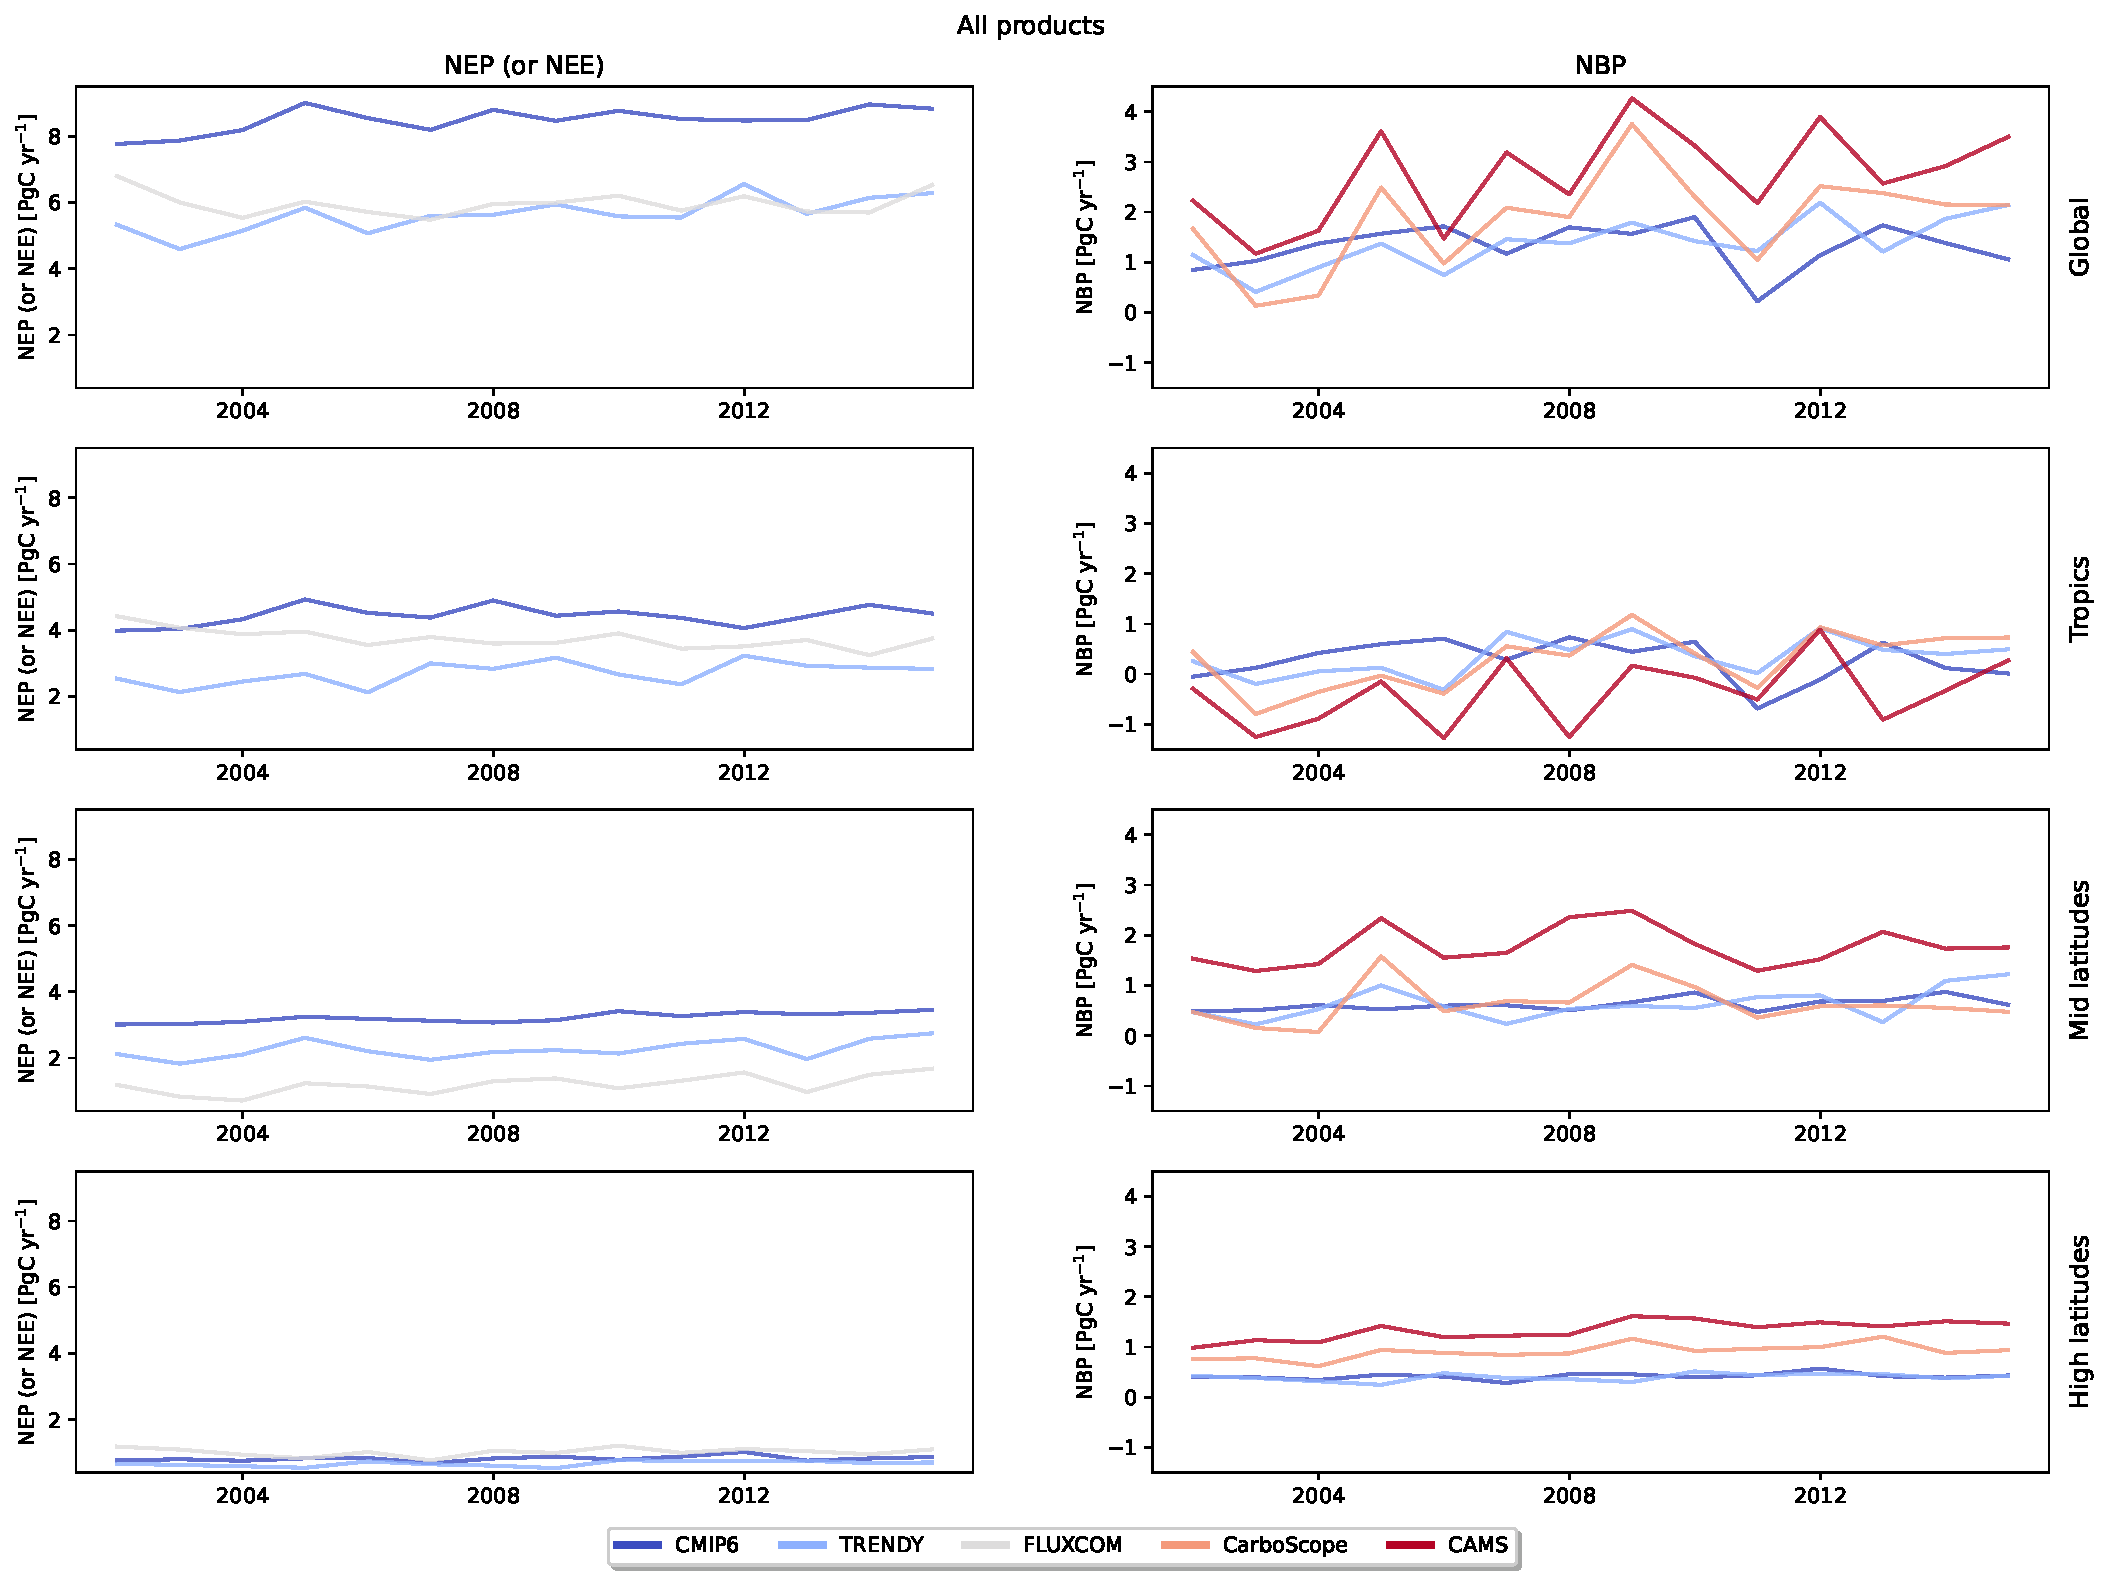
\includegraphics[width=1.0\linewidth]{Images/Allproducts_variables.pdf}
    \caption{Time series of the annual mean of NEP (NEE for X-BASE) and NBP (vertical panels) from all products, cumulated globally, in the tropics, mid-latitudes, and high latitudes (horizontal panels). Colors indicate the different products.}
    \label{fig:vars_allprod}
\end{figure}
  
\newpage
\section{Model weights}
  
\begin{figure}[!htb]
    \centering
    
\includegraphics[width=1.0\linewidth]{Images/CMIP6_FLUXCOM_weights.pdf}
    \caption{Spatial weights of NEP CMIP6 models to calculate the ensemble model average derived from X-BASE (NEE). Diverging color tables indicate whether the model contributes more or less than 1/8, where 8 is the number of models.}
    \label{fig:weights_CMIP6-FLUXCOMX}
\end{figure}
  

%\newpage
\begin{figure}[!htb]
    \centering
    
\includegraphics[width=1.0\linewidth]{Images/CMIP6_CarboScope_weights.pdf}
    \caption{Spatial weights of NBP CMIP6 models to calculate the ensemble model average derived from CarboScope. Diverging color tables indicate whether the model contributes more or less than 1/8, where 8 is the number of models.}
    \label{fig:weights_CMIP6-CarboScope}
\end{figure}

% \newpage

\begin{figure}[!htb]
    \centering
    \includegraphics[width=1.0\linewidth]{Images/TRENDY_FLUXCOM_weights.pdf}
    \caption{Spatial weights of NEP TRENDY models to calculate the ensemble model derived from X-BASE (NEE). Diverging color tables indicate whether the model contributes more or less than 1/20, where 20 is the number of models.}
    \label{fig:weights_TRENDY-FLUXCOMX}
\end{figure}

%\newpage

\begin{figure}[!h]
    \centering
    \includegraphics[width=1.0\linewidth]{Images/TRENDY_CarboScope_weights.pdf}
    \caption{Spatial weights of NBP TRENDY models to calculate the ensemble model derived from CarboScope. Diverging color tables indicate whether the model contributes more or less than 1/18, where 18 is the number of models.}
    \label{fig:weights_TRENDY-CarboScope}
\end{figure}

\newpage
  
\section{Supplementary results}

\begin{figure}[ht]
    \centering
    
\includegraphics[width=1.0\linewidth]{Images/CMIP6_NEP_NBP_CS_map_latitude_mean.pdf}
    \caption{Carbon Sequestration (CS) spatial patterns based on NEP (a,b) and NBP (c,d) from CMIP6 models (1850-2014). a,c) Global distributions of CS based on the weighted ensemble average of 8 CMIP6 models, and b,d) latitudinal CS profiles for individual CMIP6 models (colored lines) and their ensemble average (black line). The vertical dashed lines in b and c represent null values of CS, and the shadow areas indicate two standard deviations from the spatial mean. Horizontal dotted lines define the latitudinal regions (tropics, mid latitudes, and high latitudes). Note that the color bar scales differ between panels a and c, as well as the scale of the x-axis in b and d.}
    \label{fig:CMIP6_NEP_NBP_map}
\end{figure}

\begin{figure}[ht]
    \centering
    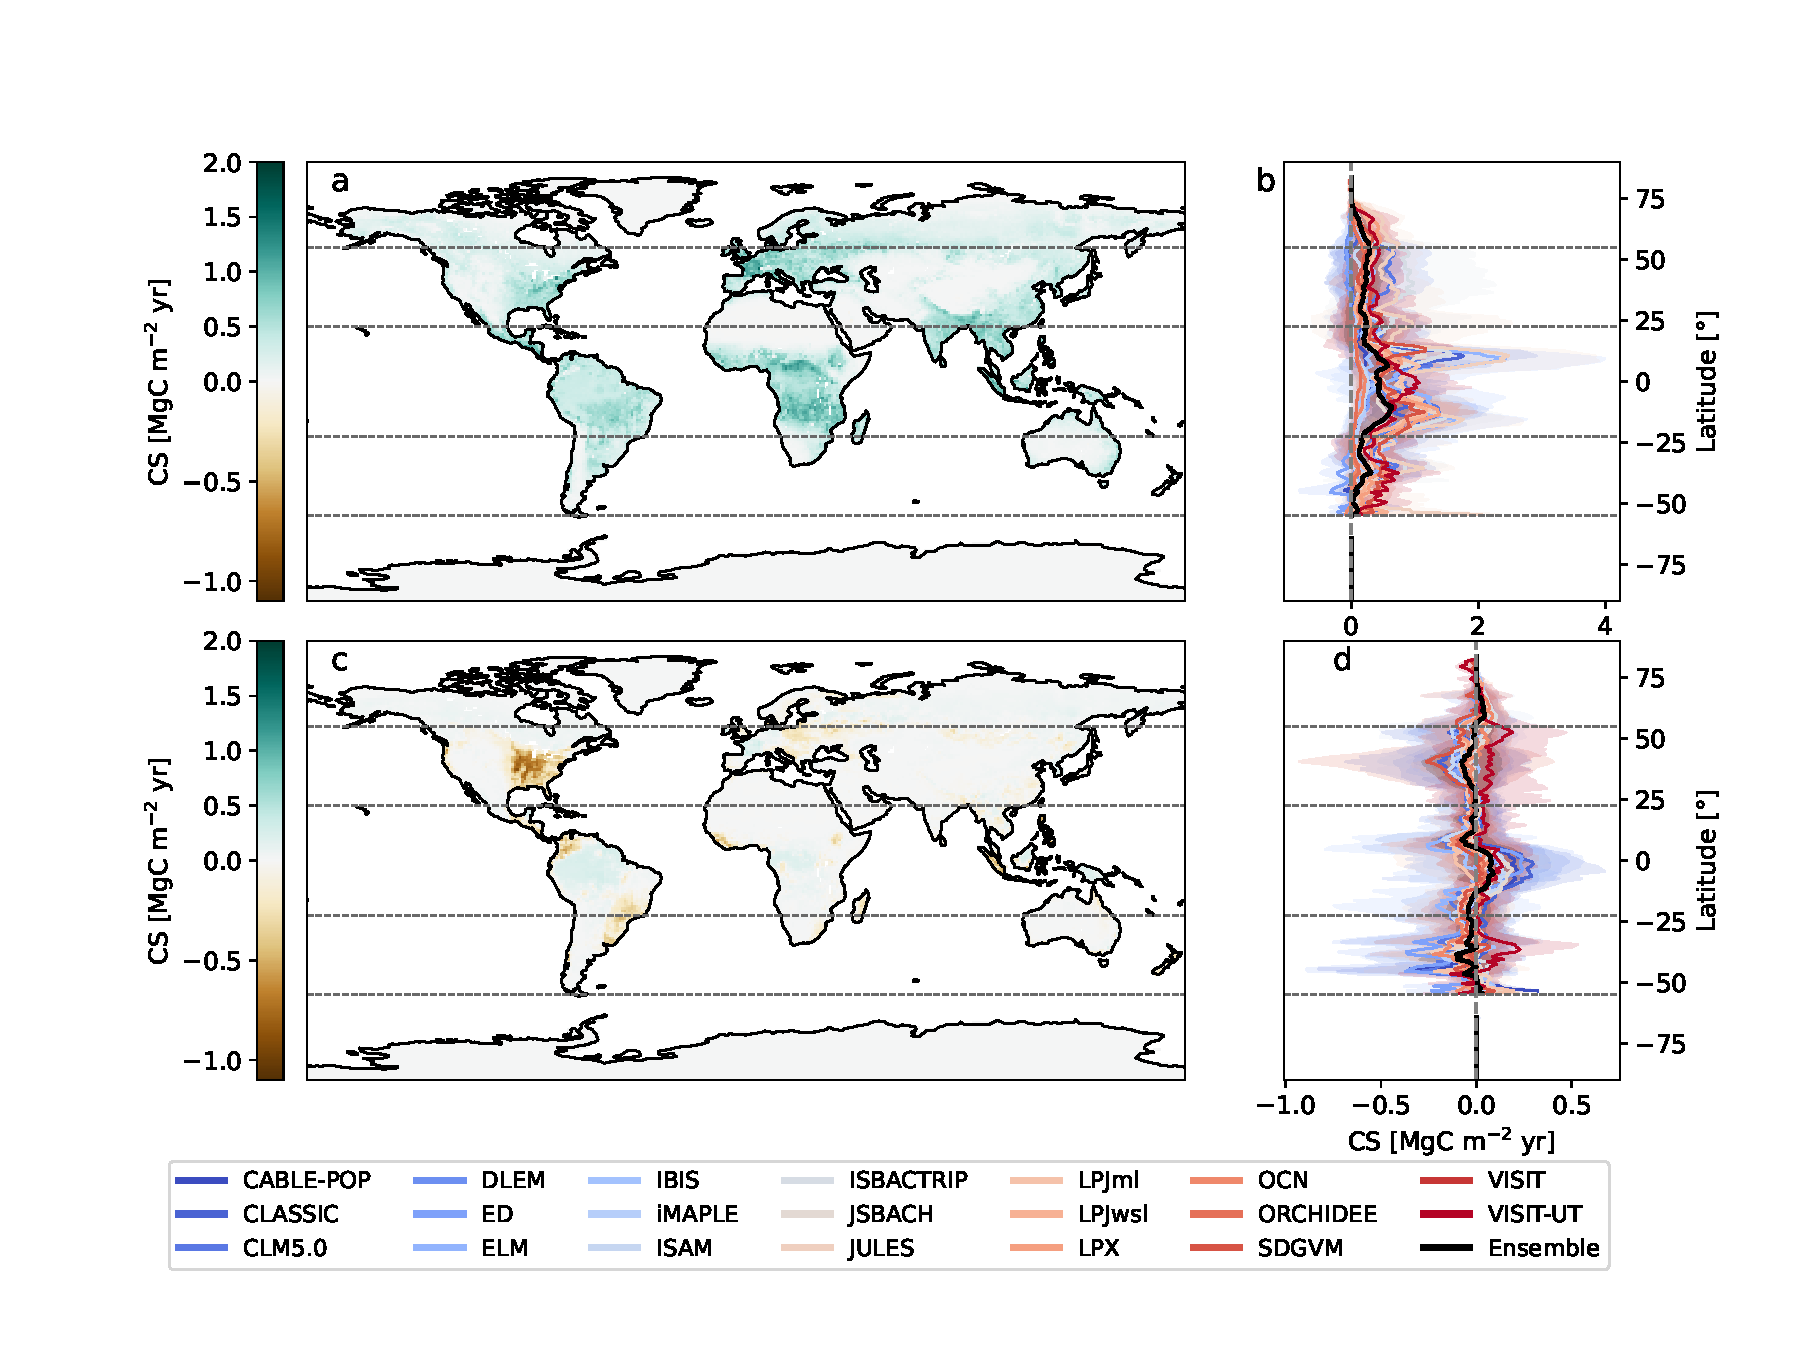
\includegraphics[width=1.0\linewidth]{Images/TRENDY_NEP_NBP_CS_map_latitude_mean.pdf}
    \caption{Carbon Sequestration (CS) spatial patterns based on NEP (a,b) and NBP (c,d) from CMIP6 models (1850-2014). a,c) Global distributions of CS based on the weighted ensemble average of 8 CMIP6 models, and b,d) latitudinal CS profiles for individual CMIP6 models (colored lines) and their ensemble average (black line). The vertical dashed lines in b and c represent null values of CS, and the shadow areas indicate two standard deviations from the spatial mean. Horizontal dotted lines define the latitudinal regions (tropics, mid latitudes, and high latitudes). Note that the color bar scales differ between panels a and c, as well as the scale of the x-axis in b and d.}
    \label{fig:TRENDY_NEP_NBP_map}
\end{figure}

\begin{table}
\label{Table:CSdiff_NEP_NBPmodels}
\caption{CS values and differences between calculations based on NEP and NBP for CMIP6 and TRENDY during 1850-2014.}
\centering
\begin{tabular}{lcccc}
\hline
\multicolumn{5}{c}{\textbf{CMIP6}}                                                                                       \\ \hline
\textbf{}                         & \textbf{Global}      & \textbf{Tropics}     & \textbf{Mid latitudes} & \textbf{High latitudes} \\
\textbf{CS NEP {[}PgC yr{]}}      & 72518              & 42810              & 25621                & 4088                 \\
\textbf{CS NBP {[}PgC yr{]}}      & -2841             & -912             & -1752               & -177               \\ \hline
\textbf{Difference  {[}PgC yr{]}} & \textbf{75359}     & \textbf{43722}     & \textbf{27373}       & \textbf{4265}        \\ \hline
                                  & \multicolumn{1}{l}{} & \multicolumn{1}{l}{} & \multicolumn{1}{l}{}   & \multicolumn{1}{l}{}    \\ \hline
\multicolumn{5}{c}{\textbf{TRENDY}}                                                                                       \\ \hline
\textbf{}                         & \textbf{Global}      & \textbf{Tropics}     & \textbf{Mid latitudes} & \textbf{High latitudes} \\
\textbf{CS NEP {[}PgC yr{]}}      & 35410               & 19028               & 12943                 & 3439                   \\
\textbf{CS NBP {[}PgC yr{]}}      & -1114               & 281                & -1881                  & 486                   \\ \hline
\textbf{Difference  {[}PgC yr{]}} & \textbf{36524}      & \textbf{18747}      & \textbf{14824}        & \textbf{2953}          \\ \hline
                                  & \multicolumn{1}{l}{} & \multicolumn{1}{l}{} & \multicolumn{1}{l}{}   & \multicolumn{1}{l}{}    \\
\end{tabular}
\end{table}
  
\begin{table}
\label{Table:CSdiff_NEP_NBP}
\caption{CS values and differences between calculations based on NEP and NBP for all products during 2001-2014.}
\centering
\begin{tabular}{lcccc}
\hline
\multicolumn{5}{c}{\textbf{CMIP6}}                                                                                       \\ \hline
\textbf{}                         & \textbf{Global}      & \textbf{Tropics}     & \textbf{Mid latitudes} & \textbf{High latitudes} \\
\textbf{CS NEP {[}PgC yr{]}}      & 820.11	             & 426.78	             & 310.86	                 & 82.47                 \\
\textbf{CS NBP {[}PgC yr{]}}      & 139.41	             & 33.17	            & 62.57                     & 43.67              \\ \hline
\textbf{Difference  {[}PgC yr{]}} & \textbf{680.70}     & \textbf{393.61}     & \textbf{248.29}       & \textbf{38.80}        \\ \hline
                                  & \multicolumn{1}{l}{} & \multicolumn{1}{l}{} & \multicolumn{1}{l}{}   & \multicolumn{1}{l}{}    \\ \hline
\multicolumn{5}{c}{\textbf{TRENDY}}                                                                                       \\ \hline
\textbf{}                         & \textbf{Global}      & \textbf{Tropics}     & \textbf{Mid latitudes} & \textbf{High latitudes} \\
\textbf{CS NEP {[}PgC yr{]}}      & 535.83	             & 251.86            	& 217.09	             & 66.88                   \\
\textbf{CS NBP {[}PgC yr{]}}      & 124.61	             & 24.02	            & 59.82	                 & 40.78                 \\ \hline
\textbf{Difference  {[}PgC yr{]}} & \textbf{411.22}      & \textbf{227.84}      & \textbf{157.27}        & \textbf{26.11}          \\ \hline
                                  & \multicolumn{1}{l}{} & \multicolumn{1}{l}{} & \multicolumn{1}{l}{}   & \multicolumn{1}{l}{}    \\
\hline
\multicolumn{5}{c}{\textbf{X-BASE}}                                                                                       \\ \hline
\textbf{}                         & \textbf{Global}      & \textbf{Tropics}     & \textbf{Mid latitudes} & \textbf{High latitudes} \\
\textbf{CS NEE {[}PgC yr{]}}      & 5591.15	             & 372.17	            & 114.39	             & 104.60
                 \\ \hline
                                  & \multicolumn{1}{l}{} & \multicolumn{1}{l}{} & \multicolumn{1}{l}{}   & \multicolumn{1}{l}{}    \\
                                    \hline
\multicolumn{5}{c}{\textbf{CarboScope}}                                                                                       \\ \hline
\textbf{}                         & \textbf{Global}      & \textbf{Tropics}     & \textbf{Mid latitudes} & \textbf{High latitudes} \\
\textbf{CS NBP {[}PgC yr{]}}      & 163.69	             & 12.88	            & 67.02	                 & 83.79
                  \\ \hline
                                  & \multicolumn{1}{l}{} & \multicolumn{1}{l}{} & \multicolumn{1}{l}{}   & \multicolumn{1}{l}{}    \\
                                    \hline
\multicolumn{5}{c}{\textbf{CAMS}}                                                                                       \\ \hline
\textbf{}                         & \textbf{Global}      & \textbf{Tropics}     & \textbf{Mid latitudes} & \textbf{High latitudes} \\
\textbf{CS NBP {[}PgC yr{]}}      & 247.63	             & -43.70	            & 169.74	             & 121.60            \\ \hline


\end{tabular}
\end{table}


\begin{figure}
    \centering
    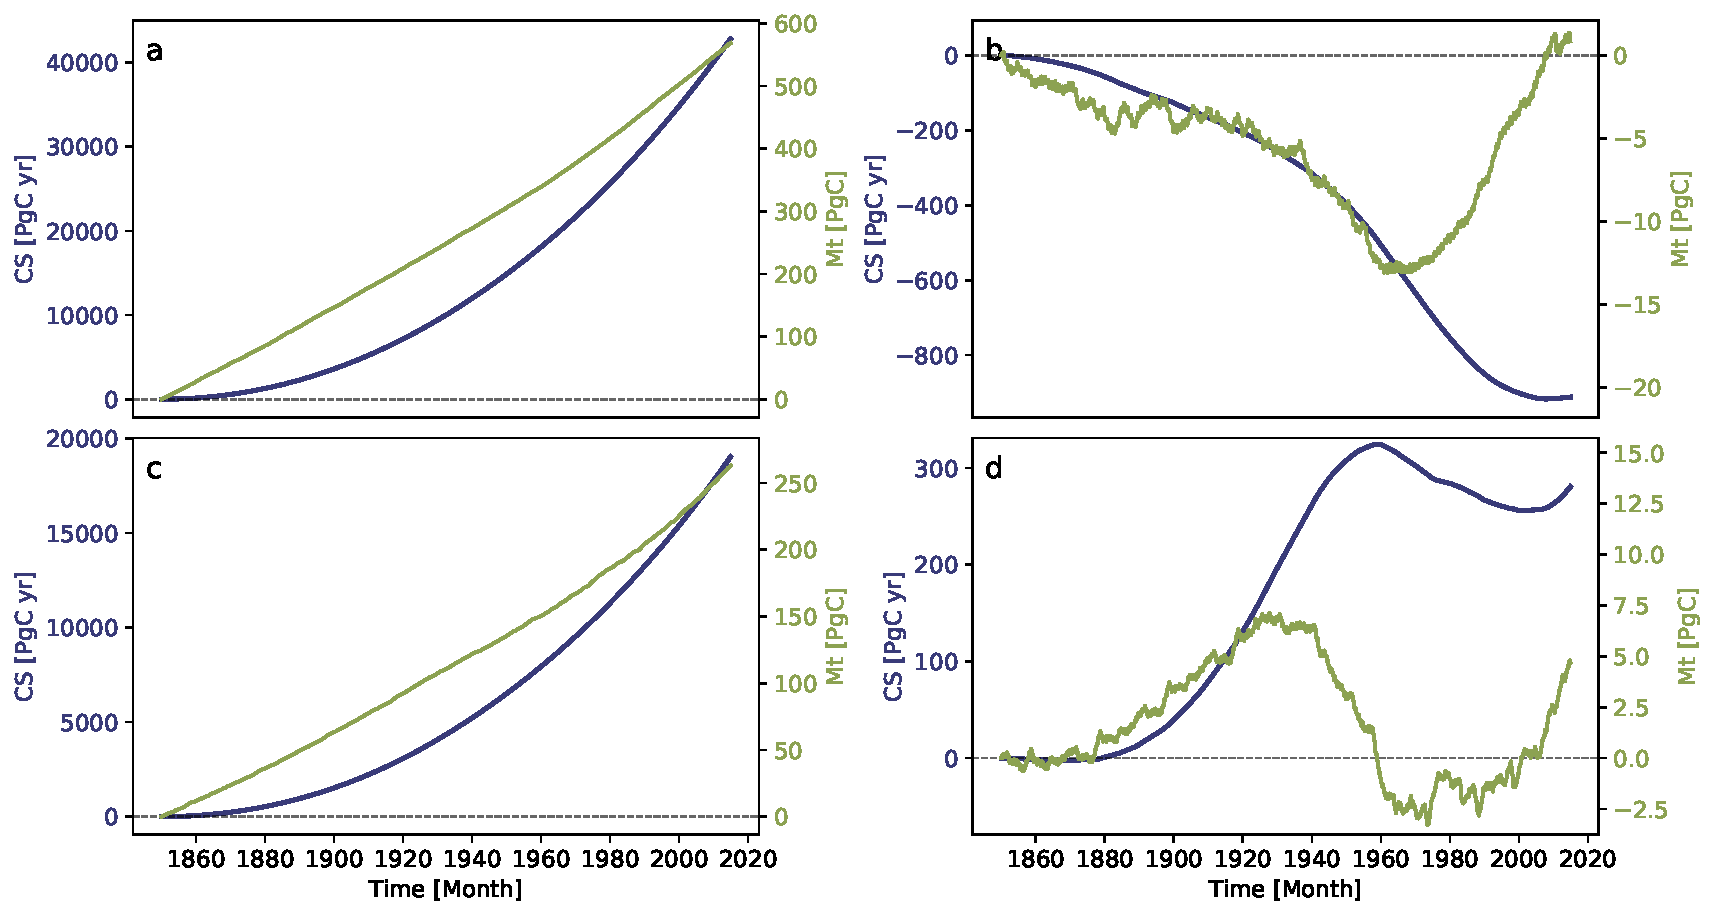
\includegraphics[width=1\linewidth]{Images/CMIP6_TRENDY_comparison_CS_Mt.pdf}
    \caption{Carbon sequestration (CS; purple line) and carbon mass or stocks (Mt; green line) derived from NEP (a, c) and NBP (b, d) outputs of CMIP6 (a, b) and TRENDY (c, d). Note that the axis ranges differ across panels to highlight the distinct information represented by CS and Mt. Dotted horizontal lines denote zero values for both CS and Mt.}
    \label{fig:CSvsMt}
\end{figure}

  
\begin{figure}
    \centering
    
\includegraphics[width=1.0\linewidth]{Images/Comparison_CS_maps_NEP.pdf}
    \caption{Spatial CS values obtained from NEP (or NEE) from a) CMIP6, b) TRENDY, and c) X-BASE from 2001-2014. Colored lines in a) and b) represent individual models; the black line is their ensemble. The dotted lines represent null carbon sequestration, and the shadow areas are two standard deviations from the mean.}
    \label{fig:LatCS_NEP}
\end{figure}

  
\begin{figure}
    \centering
    
\includegraphics[width=1.0\linewidth]{Images/Comparison_CS_maps_NBP.pdf}
    \caption{Spatial CS values obtained from NBP from a) CMIP6, b) TRENDY, c) CarboScope, and d) CAMS from 2001-2014. Colored lines in a) and b) represent individual models; the black line is their ensemble. The dotted lines represent null carbon sequestration, and the shadow areas are two standard deviations from the mean.}
    \label{fig:LatCS_NBP}
\end{figure}


\begin{figure}
    \centering
    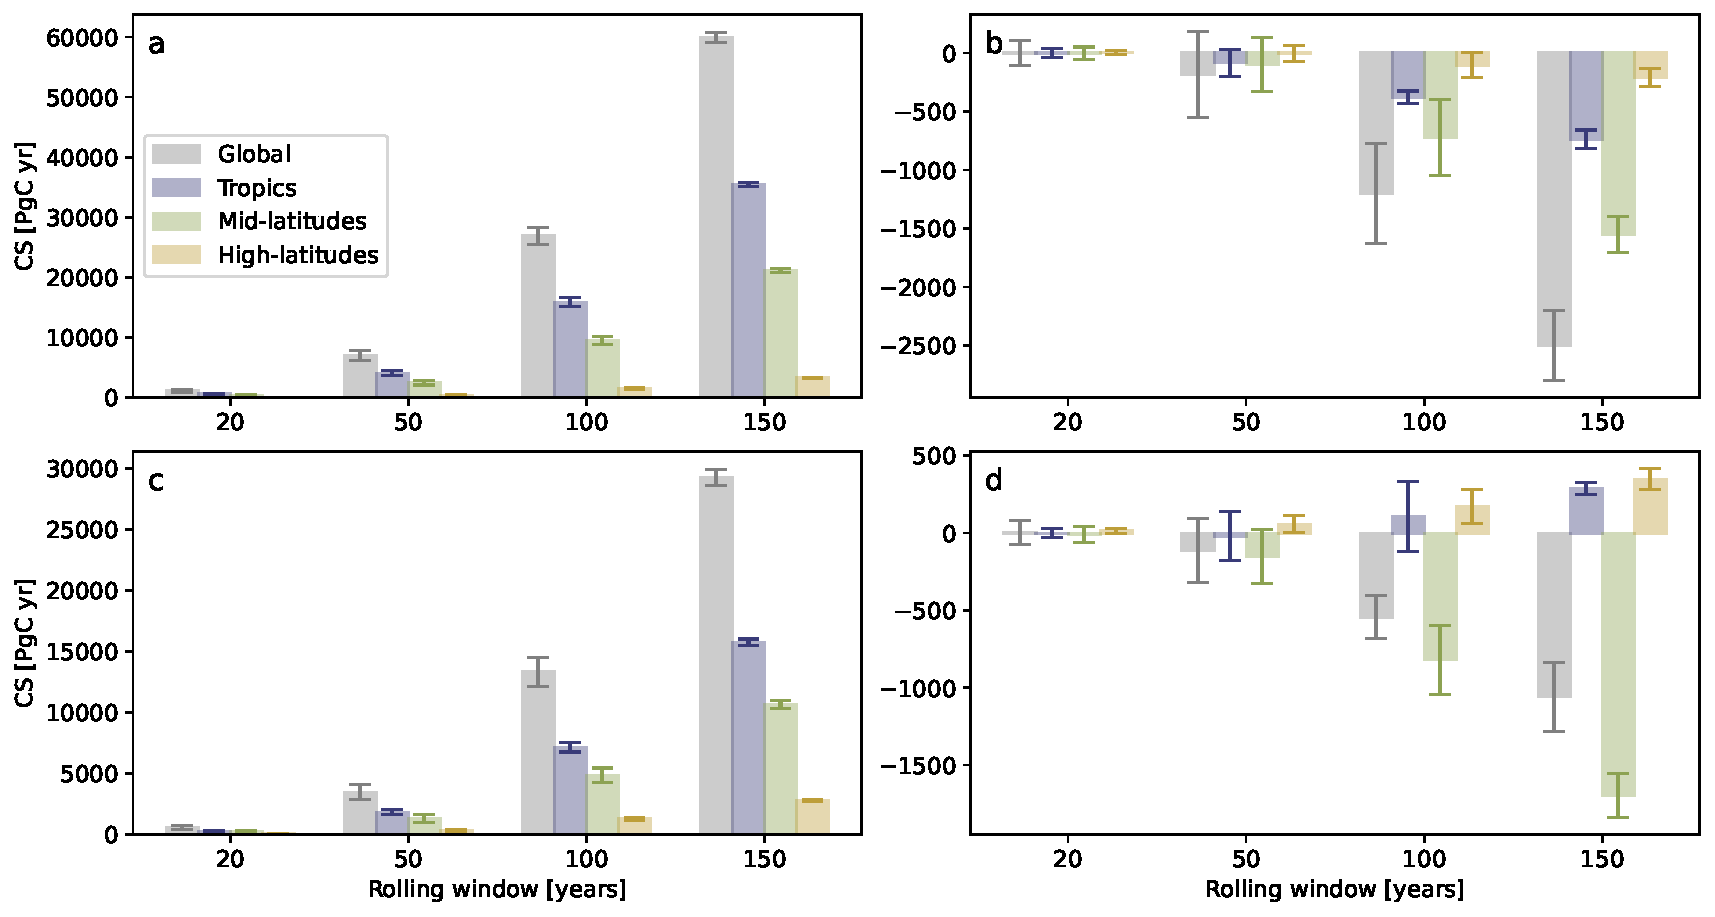
\includegraphics[width=1.0\linewidth]{Images/Rolling_window_CS.pdf}
    \caption{Variations in carbon sequestration (CS) accumulated over rolling windows ranging from 20 to 150 years, with corresponding standard deviations, for NEP (a,c) and NBP (b,d) from the CMIP (a, b) and TRENDY (c, d) ensembles. Each panel uses a different vertical scale.}
    \label{fig:roll_window_t0}
\end{figure}








% %%% Add this line AFTER all your figures and tables
\FloatBarrier

% % \movie{Type legend for the movie here.}

% % \movie{Type legend for the other movie here. Adding longer text to show what happens, to decide on alignment and/or indentations.}

% % \movie{A third movie, just for kicks.}

% % \dataset{dataset_one.txt}{Type or paste legend here.}

% % \dataset{dataset_two.txt}{Type or paste legend here. Adding longer text to show what happens, to decide on alignment and/or indentations for multi-line or paragraph captions.}

\bibliographystyle{abbrvnat}
\bibliography{biblio}

\end{document}
